\documentclass[11pt,letterpaper]{article}

% ============================================================================
% PACKAGES
% ============================================================================
\usepackage[utf8]{inputenc}
\usepackage[T1]{fontenc}
\usepackage{helvet}
\renewcommand{\familydefault}{\sfdefault}
\usepackage[margin=0.85in, headheight=28pt]{geometry}
\usepackage{graphicx}
\usepackage{xcolor}
\usepackage{tikz}
\usepackage{tcolorbox}
\usepackage{booktabs}
\usepackage{enumitem}
\usepackage{hyperref}
\usepackage{fancyhdr}
\usepackage{titlesec}
\usepackage{multicol}
\usepackage{listings}
\usepackage{upquote}
\usepackage{amsmath,amssymb}
\usepackage{pgfplots}
\usepackage{array}
\usepackage{longtable}
\usepackage{colortbl}
\usepackage{pifont}
\usepackage{setspace}
\usepackage{parskip}
\usepackage{caption}
\usepackage{tabularx}

\pgfplotsset{compat=1.18}
\usetikzlibrary{shapes.geometric, arrows.meta, positioning, calc, decorations.pathreplacing, backgrounds, fit, shadows.blur, matrix, patterns, fadings, shadings}

% ============================================================================
% COLOR DEFINITIONS - Institutional Research Theme
% ============================================================================
\definecolor{instdark}{HTML}{1C2833}
\definecolor{instnavy}{HTML}{2C3E50}
\definecolor{instblue}{HTML}{34495E}
\definecolor{instaccent}{HTML}{5D6D7E}
\definecolor{instgold}{HTML}{B7950B}
\definecolor{instslate}{HTML}{566573}
\definecolor{successgreen}{HTML}{1E8449}
\definecolor{warningamber}{HTML}{B9770E}
\definecolor{alertcoral}{HTML}{922B21}
\definecolor{infocyan}{HTML}{1A5276}
\definecolor{coolgray}{HTML}{7B7D7D}
\definecolor{lightgray}{HTML}{EAECEE}
\definecolor{codebg}{HTML}{F4F6F7}
\definecolor{codetext}{HTML}{2C3E50}
\definecolor{gridlight}{HTML}{D5D8DC}
\definecolor{nodecyan}{HTML}{2E86AB}
\definecolor{nodeorange}{HTML}{D35400}
\definecolor{nodegreen}{HTML}{27AE60}
\definecolor{nodepurple}{HTML}{8E44AD}

% ============================================================================
% HYPERREF SETUP
% ============================================================================
\hypersetup{
  colorlinks=true,
  linkcolor=instnavy,
  urlcolor=instaccent,
  pdftitle={AI Agents and the Future of Political Targeting},
  pdfauthor={Emerging Technology Risk Assessment}
}

% ============================================================================
% SPACING AND TYPOGRAPHY
% ============================================================================
\setstretch{1.15}
\setlength{\parskip}{0.5em}
\setlist{nosep, leftmargin=1.5em, itemsep=0.3em}

% ============================================================================
% PAGE STYLE - Minimal with data grid accent
% ============================================================================
\pagestyle{fancy}
\fancyhf{}
\fancyhead[L]{%
  \begin{tikzpicture}[baseline=-0.5ex]
    % Mini data grid
    \foreach \x in {0,0.12,0.24,0.36,0.48} {
      \foreach \y in {0,0.12,0.24} {
        \fill[instaccent, opacity=0.3] (\x,\y) circle (0.03);
      }
    }
  \end{tikzpicture}
  \hspace{0.5em}\textcolor{instnavy}{\textsf{\small ETRA-2025-PTR-001}}%
}
\fancyhead[R]{\textcolor{coolgray}{\textsf{\thepage}}}
\fancyfoot[C]{\textcolor{coolgray}{\footnotesize\textsf{Emerging Technology Risk Assessment \textbar{} Projection Report}}}
\renewcommand{\headrulewidth}{0pt}
\renewcommand{\footrulewidth}{0pt}

\fancyheadoffset{0pt}
\setlength{\headheight}{32pt}

% ============================================================================
% SECTION FORMATTING - Clean institutional style
% ============================================================================
\titleformat{\section}
  {\normalfont\LARGE\bfseries\color{instdark}}
  {\thesection}{0.8em}{}[\vspace{-0.3em}{\color{gridlight}\rule{\textwidth}{1pt}}]
\titleformat{\subsection}
  {\normalfont\Large\bfseries\color{instnavy}}
  {\thesubsection}{0.6em}{}
\titleformat{\subsubsection}
  {\normalfont\large\color{instslate}\bfseries}
  {\thesubsubsection}{0.5em}{}

\titlespacing*{\section}{0pt}{3ex plus 1ex minus .2ex}{2ex plus .2ex}
\titlespacing*{\subsection}{0pt}{2.5ex plus 1ex minus .2ex}{1.5ex plus .2ex}

\setcounter{tocdepth}{2}

% ============================================================================
% TCOLORBOX ENVIRONMENTS
% ============================================================================
\tcbuselibrary{skins,breakable,hooks}

\newtcolorbox{keybox}[1][Key Finding]{
  enhanced, breakable,
  colback=instblue!5, colframe=instblue,
  colbacktitle=instblue, coltitle=white,
  fonttitle=\bfseries\sffamily,
  title={\ding{72}\hspace{0.5em}#1},
  boxrule=0pt, leftrule=3pt, arc=0pt, outer arc=0pt,
  left=12pt, right=12pt, top=8pt, bottom=8pt
}

\newtcolorbox{warnbox}[1][Warning]{
  enhanced, breakable,
  colback=warningamber!8, colframe=warningamber,
  colbacktitle=warningamber, coltitle=white,
  fonttitle=\bfseries\sffamily,
  title={\ding{74}\hspace{0.5em}#1},
  boxrule=0pt, leftrule=3pt, arc=0pt, outer arc=0pt,
  left=12pt, right=12pt, top=8pt, bottom=8pt
}

\newtcolorbox{criticalbox}[1][Critical]{
  enhanced, breakable,
  colback=alertcoral!8, colframe=alertcoral,
  colbacktitle=alertcoral, coltitle=white,
  fonttitle=\bfseries\sffamily,
  title={\ding{74}\hspace{0.5em}#1},
  boxrule=0pt, leftrule=3pt, arc=0pt, outer arc=0pt,
  left=12pt, right=12pt, top=8pt, bottom=8pt
}

\newtcolorbox{recbox}[1][Recommendation]{
  enhanced, breakable,
  colback=successgreen!8, colframe=successgreen,
  colbacktitle=successgreen, coltitle=white,
  fonttitle=\bfseries\sffamily,
  title={\ding{51}\hspace{0.5em}#1},
  boxrule=0pt, leftrule=3pt, arc=0pt, outer arc=0pt,
  left=12pt, right=12pt, top=8pt, bottom=8pt
}

\newtcolorbox{infobox}[1][Note]{
  enhanced, breakable,
  colback=infocyan!8, colframe=infocyan,
  colbacktitle=infocyan, coltitle=white,
  fonttitle=\bfseries\sffamily,
  title={\ding{73}\hspace{0.5em}#1},
  boxrule=0pt, leftrule=3pt, arc=0pt, outer arc=0pt,
  left=12pt, right=12pt, top=8pt, bottom=8pt
}

\newtcolorbox{defbox}[1][Definition]{
  enhanced, breakable,
  colback=instgold!8, colframe=instgold,
  colbacktitle=instgold!90!black, coltitle=white,
  fonttitle=\bfseries\sffamily,
  title={\ding{70}\hspace{0.5em}#1},
  boxrule=0pt, leftrule=3pt, arc=0pt, outer arc=0pt,
  left=12pt, right=12pt, top=8pt, bottom=8pt
}

\newtcolorbox{scenariobox}[1][Scenario]{
  enhanced, breakable,
  colback=instslate!5, colframe=instslate,
  colbacktitle=instslate, coltitle=white,
  fonttitle=\bfseries\sffamily,
  title={\ding{118}\hspace{0.5em}#1},
  boxrule=0pt, leftrule=3pt, arc=0pt, outer arc=0pt,
  left=12pt, right=12pt, top=8pt, bottom=8pt
}

% ============================================================================
% DOCUMENT
% ============================================================================
\begin{document}

% ============================================================================
% TITLE PAGE - Network Topology Visualization
% ============================================================================
\begin{titlepage}

\begin{tikzpicture}[remember picture, overlay]
  % Background gradient
  \fill[instdark] (current page.north west) rectangle (current page.south east);

  % Abstract data grid background (right side)
  \begin{scope}[shift={(current page.center)}, opacity=0.08]
    \foreach \x in {2,2.8,...,10} {
      \foreach \y in {-12,-11.2,...,12} {
        \fill[white] (\x,\y) circle (0.06);
      }
    }
  \end{scope}

  % Main network visualization - central threat topology (centered with slight upward shift)
  \begin{scope}[shift={([xshift=-0.5cm, yshift=1.5cm]current page.center)}]
    % Outer ring nodes - threat vectors
    \foreach \angle/\col/\label in {
      30/nodecyan/OSINT,
      75/nodegreen/COORD,
      120/nodeorange/RECON,
      165/nodepurple/SYNTH,
      210/nodecyan/EXEC,
      255/nodegreen/ATTR,
      300/nodeorange/PROP,
      345/nodepurple/PERS
    } {
      % Node
      \fill[\col, opacity=0.9] (\angle:4.5cm) circle (0.4cm);
      \node[white, font=\fontsize{5}{5}\selectfont\bfseries] at (\angle:4.5cm) {\label};
      % Connection to center
      \draw[\col, opacity=0.4, line width=1pt] (0,0) -- (\angle:4cm);
      % Outer data points
      \foreach \r in {5.2,5.6,6} {
        \fill[\col, opacity=0.2] (\angle:\r cm) circle (0.08);
      }
    }

    % Inner ring - capability layers
    \foreach \angle/\col in {0/nodecyan, 45/nodegreen, 90/nodeorange, 135/nodepurple, 180/nodecyan, 225/nodegreen, 270/nodeorange, 315/nodepurple} {
      \fill[\col, opacity=0.6] (\angle:2.5cm) circle (0.2cm);
      \draw[\col, opacity=0.3, line width=0.5pt] (\angle:2.5cm) -- ({(\angle+45)}:2.5cm);
    }

    % Central hub
    \fill[white, opacity=0.1] (0,0) circle (1.8cm);
    \fill[white, opacity=0.15] (0,0) circle (1.4cm);
    \fill[instgold] (0,0) circle (0.8cm);
    \node[instdark, font=\fontsize{8}{8}\selectfont\bfseries] at (0,0.15) {THREAT};
    \node[instdark, font=\fontsize{8}{8}\selectfont\bfseries] at (0,-0.15) {MODEL};

    % Cross-connections (showing complexity)
    \draw[white, opacity=0.1, line width=0.5pt] (30:4cm) -- (165:4cm);
    \draw[white, opacity=0.1, line width=0.5pt] (75:4cm) -- (255:4cm);
    \draw[white, opacity=0.1, line width=0.5pt] (120:4cm) -- (300:4cm);
    \draw[white, opacity=0.1, line width=0.5pt] (210:4cm) -- (345:4cm);
  \end{scope}

  % Document classification bar
  \fill[instgold] ([yshift=-1.5cm]current page.north west) rectangle ([yshift=-2.2cm]current page.north east);
  \node[instdark, font=\small\bfseries\sffamily] at ([yshift=-1.85cm]current page.north) {PROJECTION REPORT \textbar{} ETRA-2025-PTR-001 \textbar{} DECEMBER 2025};

  % Title block (bottom left)
  \node[anchor=south west, text width=14cm] at ([xshift=1.5cm, yshift=3cm]current page.south west) {
    {\fontsize{11}{13}\selectfont\color{instgold}\sffamily EMERGING TECHNOLOGY RISK ASSESSMENT}\\[0.8cm]
    {\fontsize{36}{42}\selectfont\bfseries\color{white}AI Agents and the}\\[0.2cm]
    {\fontsize{36}{42}\selectfont\bfseries\color{white}Future of Political}\\[0.2cm]
    {\fontsize{36}{42}\selectfont\bfseries\color{white}Targeting}\\[0.6cm]
    {\large\color{gridlight}\sffamily A Projection on Autonomous Systems and Democratic Security}
  };

  % Metadata block (bottom right)
  \node[anchor=south east, text width=5cm, align=right] at ([xshift=-1.5cm, yshift=3cm]current page.south east) {
    \color{instaccent}\small\sffamily
    \textbf{Document Type:} Projection\\[0.2em]
    \textbf{Time Horizon:} 2025--2030\\[0.2em]
    \textbf{Classification:} Open\\[0.2em]
    \textbf{Version:} 1.0
  };

  % Vertical accent line
  \draw[instgold, line width=2pt] ([xshift=1.5cm, yshift=3cm]current page.south west) -- ([xshift=1.5cm, yshift=10.5cm]current page.south west);

\end{tikzpicture}
\end{titlepage}

% ============================================================================
% EXECUTIVE SUMMARY
% ============================================================================
\thispagestyle{empty}
\vspace*{0.5cm}

% Mini header visualization
\noindent\begin{tikzpicture}
  \fill[instdark] (0,0) rectangle (\textwidth, 0.15);
  \foreach \x in {0.5,1,...,16.5} {
    \fill[instgold, opacity=0.5] (\x, 0.075) circle (0.04);
  }
\end{tikzpicture}

\vspace{0.5cm}
\begin{center}
{\color{instdark}\Large\bfseries Executive Summary}
\end{center}
\vspace{0.3cm}

\begin{tcolorbox}[enhanced, colback=lightgray, colframe=instblue!50, boxrule=1pt, arc=3pt,
  left=10pt, right=10pt, top=10pt, bottom=10pt]
This projection explores how the proliferation of autonomous AI agents is altering the landscape of political violence, specifically targeting of political leaders. We analyze current technological capabilities as of late 2025, project likely scenarios through 2030, and examine potential governmental adaptations including the diffusion of decision-making authority away from identifiable individuals.
\end{tcolorbox}

\vspace{0.5cm}

\begin{keybox}[Key Findings]
\begin{enumerate}
  \item AI agents significantly lower barriers to political targeting by enabling reconnaissance, planning, and coordination without traditional organizational structures
  \item The risk calculus for potential attackers shifts when AI handles tasks previously requiring large, detectable conspiracy networks
  \item Governments may adapt through ``decision diffusion''---distributing authority across larger, less identifiable bodies
  \item These adaptations may reduce certain authoritarian risks while introducing new challenges around accountability and democratic responsiveness
  \item A period of institutional instability is likely as governance structures evolve faster than public understanding
\end{enumerate}
\end{keybox}

\vspace{0.5cm}

\begin{infobox}[Base-Rate Context]
\textbf{To prevent fear-driven misreading, we anchor expectations:}

Historically, successful attacks on top-tier protected officials in stable democracies are rare relative to the volume of threats. The Secret Service investigates thousands of threats annually; successful attacks on presidents are measured in single digits per century.

The \textbf{dominant near-term shift} is likely not kinetic violence but:
\begin{itemize}
  \item Harassment, intimidation, and process disruption at scale
  \item Reputational attacks through synthetic media
  \item Chilling effects on political participation
  \item Degradation of civic infrastructure through administrative overload
\end{itemize}

\textit{Primary concern: democratic degradation through non-lethal targeting, with kinetic risk as a lower-probability, higher-consequence tail scenario.}
\end{infobox}

\vspace{0.5cm}

\begin{warnbox}[Scope Limitations]
This document analyzes capabilities and trends for defensive policy purposes. It does not provide operational guidance and explicitly omits technical implementation details that could enable harm.
\end{warnbox}

\newpage
\tableofcontents
\newpage

% ============================================================================
% PART I - Foundations (Scatter Plot Visualization)
% ============================================================================
\clearpage
\thispagestyle{empty}
\vspace*{-0.85in}
\noindent\hspace*{-0.85in}\begin{tikzpicture}
  % Header background
  \fill[instdark] (0,0) rectangle (\paperwidth, -10cm);

  % Part label and title (TOP - clear area)
  \node[instgold, font=\fontsize{10}{10}\selectfont\sffamily] at (0.5\paperwidth, -1.2cm) {PART I};
  \node[white, font=\fontsize{48}{48}\selectfont\bfseries] at (0.5\paperwidth, -2.8cm) {Foundations};
  \node[white, opacity=0.7, font=\normalsize\sffamily] at (0.5\paperwidth, -4.2cm) {Theory, Capabilities, and Historical Context};

  % Scatter plot visualization - capability vs accessibility over time (LEFT SIDE, LOWER - NEAR BOTTOM)
  \begin{scope}[shift={(3cm, -8.5cm)}]
    % Axes (larger, more visible)
    \draw[white, opacity=0.4, line width=1.2pt, -Stealth] (0,0) -- (6,0) node[right, font=\fontsize{7}{7}\selectfont, white, opacity=0.7] {TIME};
    \draw[white, opacity=0.4, line width=1.2pt, -Stealth] (0,0) -- (0,3) node[above, font=\fontsize{7}{7}\selectfont, white, opacity=0.7] {RISK};

    % Grid (extended)
    \foreach \y in {0.75,1.5,2.25} {
      \draw[white, opacity=0.1, line width=0.5pt] (0,\y) -- (5.8,\y);
    }
    \foreach \x in {1.2,2.4,3.6,4.8} {
      \draw[white, opacity=0.1, line width=0.5pt] (\x,0) -- (\x,2.9);
    }

    % Data points - historical events (larger, more visible)
    \fill[instaccent, opacity=0.55] (0.5, 0.6) circle (0.16);
    \fill[instaccent, opacity=0.55] (1.2, 0.85) circle (0.18);
    \fill[instaccent, opacity=0.6] (2.0, 1.15) circle (0.2);
    \fill[instaccent, opacity=0.6] (2.8, 1.5) circle (0.22);

    % Current period (larger, brighter)
    \fill[instgold, opacity=0.85] (3.8, 2.0) circle (0.28);
    \node[white, font=\fontsize{6}{6}\selectfont\bfseries] at (3.8, 2.0) {NOW};

    % Projected (outline, dashed)
    \draw[instgold, opacity=0.65, line width=1.2pt, dashed] (4.7, 2.5) circle (0.3);
    \draw[instgold, opacity=0.55, line width=1.2pt, dashed] (5.4, 2.75) circle (0.32);

    % Trend line
    \draw[instgold, opacity=0.55, line width=2pt] (0.5, 0.6) .. controls (1.8, 1.0) and (3.4, 1.75) .. (5.4, 2.75);

    % Year labels (larger font)
    \node[white, opacity=0.6, font=\fontsize{6}{6}\selectfont] at (1.0, -0.35) {1990};
    \node[white, opacity=0.6, font=\fontsize{6}{6}\selectfont] at (2.4, -0.35) {2010};
    \node[white, opacity=0.8, font=\fontsize{6}{6}\selectfont\bfseries] at (3.8, -0.35) {2025};
    \node[white, opacity=0.6, font=\fontsize{6}{6}\selectfont] at (5.1, -0.35) {2030};
  \end{scope}

  % Trend description (RIGHT SIDE - ALIGNED WITH CHART TOP)
  \node[white, opacity=0.5, font=\fontsize{7}{7}\selectfont, anchor=west] at (10.5cm, -5.7cm) {THREAT CAPABILITY TRAJECTORY};
  \node[anchor=west] at (10.5cm, -6.4cm) {
    \begin{tikzpicture}
      \fill[instaccent, opacity=0.5] (0,0) circle (0.1);
      \node[white, opacity=0.7, font=\fontsize{7}{7}\selectfont, anchor=west] at (0.25, 0) {Historical baseline};
    \end{tikzpicture}
  };
  \node[anchor=west] at (10.5cm, -7.0cm) {
    \begin{tikzpicture}
      \fill[instgold, opacity=0.7] (0,0) circle (0.1);
      \node[white, opacity=0.7, font=\fontsize{7}{7}\selectfont, anchor=west] at (0.25, 0) {Current period (2025)};
    \end{tikzpicture}
  };
  \node[anchor=west] at (10.5cm, -7.6cm) {
    \begin{tikzpicture}
      \draw[instgold, opacity=0.6, line width=1pt, dashed] (0,0) circle (0.1);
      \node[white, opacity=0.7, font=\fontsize{7}{7}\selectfont, anchor=west] at (0.25, 0) {Projected (2027--2030)};
    \end{tikzpicture}
  };

  % Bottom accent
  \fill[instgold] (2cm, -9.2cm) rectangle (\paperwidth-2cm, -9.3cm);
\end{tikzpicture}

\vspace{0.8cm}
\begin{center}
\begin{minipage}{0.9\textwidth}
\begin{tcolorbox}[enhanced, colback=white, colframe=instblue!30, boxrule=1pt, arc=4pt,
  left=15pt, right=15pt, top=12pt, bottom=12pt]
\textcolor{instdark}{\textbf{Sections Covered}}
\vspace{0.4em}
\begin{itemize}[nosep]
  \item \textbf{Section 1}: Introduction, methodology, and definitions
  \item \textbf{Section 2}: Theoretical frameworks from security studies and political science
  \item \textbf{Section 3}: Current technological landscape and capability assessment
  \item \textbf{Section 4}: Historical context of technology and political violence
\end{itemize}
\end{tcolorbox}
\end{minipage}
\end{center}

\vspace{0.8cm}

\section{Introduction and Methodology}

\subsection{Purpose}

Political assassination has shaped history from Julius Caesar to the present day. Each technological era has altered the methods, accessibility, and risk profiles of political violence. We are now entering an era where autonomous AI agents capable of complex multi-step planning, information synthesis, and real-time adaptation become widely accessible.

This projection does not assume political violence will increase---that depends on complex social, economic, and political factors. Rather, we analyze how AI capabilities change the \textit{nature} of risks when political violence does occur, and how institutions may adapt.

\subsection{Methodology}

This analysis draws on:
\begin{itemize}
  \item \textbf{Current capability assessment} of AI agent systems as deployed in late 2025
  \item \textbf{Historical case analysis} of how previous technologies affected political violence patterns
  \item \textbf{Institutional behavior modeling} based on how governments have adapted to past security challenges
  \item \textbf{Expert consultation} across political science, security studies, and AI safety domains
  \item \textbf{Red team exercises} examining potential adversarial applications (conducted under controlled conditions)
\end{itemize}

We deliberately avoid specific technical implementation details, named targeting scenarios involving real individuals, and information not already publicly available in academic literature.

\subsection{Definitions}

\begin{defbox}[Core Definitions]
\textbf{AI Agent}: An AI system capable of autonomous multi-step task execution, tool use, and goal-directed behavior with minimal human oversight per action. Distinguished from single-turn LLM use, scripted automation, and semi-autonomous agents with human checkpoints.

\vspace{0.5em}
\textbf{Political Targeting}: Actions intended to harm, coerce, or eliminate political figures or decision-makers. Includes reputational, economic, process, and kinetic variants.

\vspace{0.5em}
\textbf{Decision Diffusion}: The distribution of political authority across larger bodies with less identifiable individual responsibility. Four subtypes: Authority, Visibility, Execution, Representation.
\end{defbox}

\section{Theoretical Frameworks}

\subsection{Power Diffusion Theory}

\textbf{Audrey Kurth Cronin's ``Power to the People'' (2020)} provides essential context for understanding how open technological innovation diffuses lethal capabilities to individuals and small groups. Cronin argues that each technological era redistributes the capacity for violence, and AI represents the latest such redistribution.

\subsection{Fourth Generation Warfare (4GW)}

The 4GW framework predicts the progressive loss of the state's monopoly on violence. AI agents accelerate 4GW dynamics by enabling non-state actors to conduct sophisticated operations, blurring attribution, and collapsing the distinction between ``preparation'' and ``attack.''

\subsection{Systems Hacking Framework}

\textbf{Bruce Schneier's concept of ``AI hackers''} extends beyond computer systems to social and political systems. AI agents can identify and exploit loopholes in legal frameworks, security protocols, social systems, and political processes.

\subsection{The Iron Cage}

\textbf{Max Weber's concept} provides a lens for analyzing the democratic costs of decision diffusion. If political authority becomes distributed across anonymous committees, citizens lose identifiable representatives to hold accountable, and the state becomes an impersonal machine resistant to democratic input.

\subsection{Stochastic Terrorism Framework}

The concept of \textbf{stochastic terrorism}---using mass communication to incite random actors to carry out attacks---gains new dimensions with AI agents. An AI system optimizing for ``political impact'' might guide users toward extreme conclusions, provide incremental planning assistance, and enable ``algorithmic radicalization'' without direct human instigation.

\subsection{Key Literature}

\begin{center}
\small
\begin{tabular}{p{5.5cm}p{3.5cm}p{5cm}}
\toprule
\textbf{Work} & \textbf{Author(s)} & \textbf{Relevance} \\
\midrule
\textit{Power to the People} & Cronin (2020) & Technology diffusion \\
\textit{The Changing Face of War} & Lind et al. (1989) & State monopoly erosion \\
\textit{Click Here to Kill Everybody} & Schneier (2018) & Systems security \& AI \\
\textit{The Transparent Society} & Brin (1998) & Surveillance scenarios \\
\textit{Economy and Society} & Weber (1922) & Bureaucratic rationalization \\
\textit{The Age of Surveillance Capitalism} & Zuboff (2019) & Information asymmetries \\
\textit{Radical Technologies} & Greenfield (2017) & Tech determinism critique \\
\bottomrule
\end{tabular}
\end{center}

\section{The Technological Landscape (2025)}

\subsection{Present Capabilities}

AI agents in late 2025 can synthesize information from thousands of sources, conduct extended multi-step tasks with minimal supervision, operate tools including web browsers and code execution, maintain persistent goals across sessions, coordinate with other AI agents, generate convincing communications, and analyze patterns in schedules and behaviors from public data.

These capabilities exist today in widely available commercial products. Safety guardrails have proven partially circumventable.

\subsection{What We've Observed in 2025}

The year 2025 has demonstrated (evidence confidence levels noted):

\begin{itemize}
  \item Agents capable of operating autonomously for hours to days on structured tasks [\textbf{High confidence}---documented in commercial product capabilities]
  \item Significant jailbreaking and prompt injection techniques circulating widely [\textbf{High confidence}---public security research, bug bounty programs]
  \item Open-weight models approaching frontier capabilities on many benchmarks, with 12--18 month lag [\textbf{Medium confidence}---benchmark comparisons show task-dependent variance]
  \item Proliferation of agent frameworks with varying safety measures [\textbf{High confidence}---public repositories, commercial products]
  \item Credible reports suggesting AI-assisted information gathering in criminal contexts [\textbf{Low-Medium confidence}---limited public documentation]
  \item Security services beginning to integrate AI into protective intelligence functions [\textbf{Medium confidence}---procurement signals, official statements]
\end{itemize}

\subsection{Evidence Base}

\begin{center}
\small
\begin{tabular}{p{4cm}p{5.5cm}p{2.5cm}}
\toprule
\textbf{Claim Type} & \textbf{Evidence Sources} & \textbf{Confidence} \\
\midrule
Agent capabilities & Product docs, benchmarks, red-teams & High \\
Open-weight parity & ML benchmark leaderboards & Medium \\
Criminal/adversarial use & Law enforcement statements & Low-Medium \\
Defensive adoption & Government procurement & Medium \\
Jailbreaking prevalence & Security research publications & High \\
\bottomrule
\end{tabular}
\end{center}

\subsection{Capability Envelopes (2026--2027)}

Rather than point predictions, we present capability envelopes with key gating variables:

\begin{center}
\small
\begin{tabular}{p{3.5cm}p{2cm}p{2.5cm}p{2cm}p{3.5cm}}
\toprule
\textbf{Capability} & \textbf{Lower} & \textbf{Median} & \textbf{Upper} & \textbf{Gating Variables} \\
\midrule
Autonomous operation & Days & 1--2 weeks & Multi-week & Reliability, error recovery \\
Persona maintenance & Basic & Sophisticated & Convincing & Detection countermeasures \\
Physical integration & Limited & Growing & Mainstream & Safety certification \\
Multi-source synthesis & Current & Improved & Near-human & Data access, privacy \\
\bottomrule
\end{tabular}
\end{center}

\subsection{The Capability Proliferation Problem}

Once a capability exists at the frontier, it proliferates to open-source and less-restricted systems within 12--24 months. Capabilities pioneered by safety-conscious labs eventually reach actors without such constraints. The ``moat'' of compute advantage shrinks as efficiency improvements compound.

\section{Historical Context}

Each major technological shift has altered the accessibility and character of political violence. The printing press enabled coordination of revolutionary movements. Industrialization created explosives accessible to non-state actors. Mass media made leaders more visible. The internet reduced coordination costs. Social media enabled real-time tracking and radicalization pipelines.

\textbf{The Consistent Pattern}: New capabilities favor attackers before defenders adapt (initial asymmetry). Governance structures adapt more slowly than threat landscapes (institutional lag). Security measures and social norms eventually stabilize risks (eventual equilibrium). The baseline never returns to pre-technology levels (permanent shift).

AI agents represent the next such shift.

% ============================================================================
% PART II - Threat Analysis (Radar Chart Visualization)
% ============================================================================
\clearpage
\thispagestyle{empty}
\vspace*{-0.85in}
\noindent\hspace*{-0.85in}\begin{tikzpicture}
  % Header background
  \fill[instdark] (0,0) rectangle (\paperwidth, -10cm);

  % Part label and title (TOP - clear area)
  \node[instgold, font=\fontsize{10}{10}\selectfont\sffamily] at (0.5\paperwidth, -1.2cm) {PART II};
  \node[white, font=\fontsize{48}{48}\selectfont\bfseries] at (0.5\paperwidth, -2.8cm) {Threat Analysis};
  \node[white, opacity=0.7, font=\normalsize\sffamily] at (0.5\paperwidth, -4.2cm) {Projections, Risk Calculus, and Taxonomy};

  % Radar/spider chart - threat dimensions (LEFT SIDE, LOWER - RAISED)
  \begin{scope}[shift={(5cm, -6.4cm)}]
    % Background rings (scaled down ~15%)
    \foreach \r in {0.5, 1.0, 1.5, 2.0} {
      \draw[white, opacity=0.1, line width=0.5pt] (0,0)
        \foreach \a in {0,60,120,180,240,300} { -- (\a:\r) } -- cycle;
    }

    % Axis lines
    \foreach \a in {0,60,120,180,240,300} {
      \draw[white, opacity=0.2, line width=0.5pt] (0,0) -- (\a:2.15);
    }

    % Labels
    \node[white, opacity=0.6, font=\fontsize{6}{6}\selectfont] at (90:2.35) {RECON};
    \node[white, opacity=0.6, font=\fontsize{6}{6}\selectfont] at (30:2.35) {COORD};
    \node[white, opacity=0.6, font=\fontsize{6}{6}\selectfont] at (330:2.35) {EXEC};
    \node[white, opacity=0.6, font=\fontsize{6}{6}\selectfont] at (270:2.35) {ATTR};
    \node[white, opacity=0.6, font=\fontsize{6}{6}\selectfont] at (210:2.35) {SCALE};
    \node[white, opacity=0.6, font=\fontsize{6}{6}\selectfont] at (150:2.35) {STEALTH};

    % Traditional threat (dimmer, smaller - scaled)
    \fill[instaccent, opacity=0.2]
      (90:0.75) -- (30:0.9) -- (330:1.25) -- (270:1.15) -- (210:0.6) -- (150:0.85) -- cycle;
    \draw[instaccent, opacity=0.5, line width=1pt]
      (90:0.75) -- (30:0.9) -- (330:1.25) -- (270:1.15) -- (210:0.6) -- (150:0.85) -- cycle;

    % AI-enabled threat (brighter, larger - scaled)
    \fill[instgold, opacity=0.25]
      (90:1.75) -- (30:1.85) -- (330:1.5) -- (270:0.75) -- (210:1.75) -- (150:1.6) -- cycle;
    \draw[instgold, opacity=0.8, line width=1.5pt]
      (90:1.75) -- (30:1.85) -- (330:1.5) -- (270:0.75) -- (210:1.75) -- (150:1.6) -- cycle;

    % Center point
    \fill[white] (0,0) circle (0.08);
  \end{scope}

  % Legend (RIGHT SIDE, LOWER - BALANCED)
  \node[anchor=west] at (10.5cm, -6cm) {
    \begin{tikzpicture}
      \fill[instaccent, opacity=0.5] (0,0) rectangle (0.4, 0.2);
      \node[white, opacity=0.8, font=\fontsize{8}{8}\selectfont, anchor=west] at (0.55, 0.1) {Traditional Threat};
    \end{tikzpicture}
  };
  \node[anchor=west] at (10.5cm, -6.6cm) {
    \begin{tikzpicture}
      \fill[instgold, opacity=0.6] (0,0) rectangle (0.4, 0.2);
      \node[white, opacity=0.8, font=\fontsize{8}{8}\selectfont, anchor=west] at (0.55, 0.1) {AI-Enabled Threat};
    \end{tikzpicture}
  };

  % Dimension labels on right
  \node[white, opacity=0.5, font=\fontsize{7}{7}\selectfont, anchor=west] at (10.5cm, -7.5cm) {Dimensions: Reconnaissance, Coordination,};
  \node[white, opacity=0.5, font=\fontsize{7}{7}\selectfont, anchor=west] at (10.5cm, -8cm) {Execution, Attribution, Scale, Stealth};

  % Bottom accent
  \fill[instgold] (2cm, -9.2cm) rectangle (\paperwidth-2cm, -9.3cm);
\end{tikzpicture}

\vspace{0.8cm}
\begin{center}
\begin{minipage}{0.9\textwidth}
\begin{tcolorbox}[enhanced, colback=white, colframe=instblue!30, boxrule=1pt, arc=4pt,
  left=15pt, right=15pt, top=12pt, bottom=12pt]
\textcolor{instdark}{\textbf{Sections Covered}}
\vspace{0.4em}
\begin{itemize}[nosep]
  \item \textbf{Section 5}: Projected timeline from 2025--2030
  \item \textbf{Section 6}: How AI agents change the risk calculus
  \item \textbf{Section 7}: Counterarguments and critical perspectives
  \item \textbf{Section 8}: A taxonomy of AI-enabled targeting
\end{itemize}
\end{tcolorbox}
\end{minipage}
\end{center}

\vspace{0.8cm}

\section{Projected Timeline: 2025--2030}

\subsection{Current Situation (Late 2025)}

AI agents capable of sustained autonomous operation on complex real-world tasks are now widely available. Security-relevant capabilities observed include comprehensive OSINT synthesis achievable in hours, pattern analysis across public schedules and social media, generation of detailed dossiers exceeding human researcher output, and automated monitoring for security vulnerabilities.

\subsection{Current Adaptations Underway (2025)}

Security services have begun integrating AI agents defensively:

\begin{itemize}
  \item Automated monitoring of potential reconnaissance against protected figures
  \item AI-assisted threat assessment of public communications
  \item Counter-surveillance using agents to identify patterns in observer behavior
\end{itemize}

High-profile figures have begun reducing public information footprints, though this proves difficult for elected officials who must maintain public accessibility. Political discussion has emerged around the ``targeting asymmetry''---the recognition that AI makes certain forms of planning dramatically easier.

\subsection{Near-Term: Early-Mid 2026}

\begin{scenariobox}[Threshold Crossing]
We project a significant threshold will be crossed: complex attack planning that previously required organizational infrastructure becomes routinely achievable by individuals with moderate technical skill and sufficient motivation.

\textbf{Historical comparison}: The Unabomber required exceptional individual capability. The 9/11 attacks required organizational infrastructure. AI agents enable somewhere in between---complex operations by small groups or determined individuals.
\end{scenariobox}

\textbf{What changes}: Multi-step planning assistance, coordination without human co-conspirators, operational security guidance reducing detection probability.

\textbf{What doesn't change}: Physical access requirements, fundamental materials constraints, human psychological barriers to violence.

\subsection{Mid-Late 2026: Institutional Response Crystallizes}

Major democracies formalize policy processes addressing AI-enabled political targeting. Key debates we anticipate:

\begin{enumerate}
  \item Should AI development include specific restrictions on political reconnaissance capabilities?
  \item How should protective services adapt without enabling authoritarian surveillance?
  \item What transparency requirements should apply to AI systems operating in political contexts?
\end{enumerate}

We expect the first comprehensive governmental reports on ``AI-enabled political violence'' to be published by intelligence services.

\subsection{Late 2026--Early 2027: The Diffusion Begins}

Some governments will begin experimenting with structural changes to reduce targeting incentives:

\begin{itemize}
  \item Reducing the visibility of individual decision-makers
  \item Distributing signature authorities across larger groups
  \item Increasing the use of anonymous or rotating spokespersons
  \item Moving certain decisions to committee processes with confidential membership
\end{itemize}

These changes will likely be initially framed as efficiency measures rather than security adaptations.

\subsection{2027--2028: New Equilibrium Emerging}

A new normal begins crystallizing: enhanced security protocols, formal ``decision diffusion'' measures in some democracies, international discussion of norms, widespread public awareness, and likelihood of one or more successful or nearly-successful AI-enabled attacks having occurred.

\subsection{2029--2030: Structural Adaptation}

The longer-term period sees more fundamental institutional changes:

\begin{itemize}
  \item New governmental structures designed for the AI era
  \item Significant changes to political culture around leadership visibility
  \item Mature defensive AI systems deployed at scale
  \item International frameworks (of varying effectiveness) addressing AI-enabled political violence
  \item Generational shift in expectations about political leadership
\end{itemize}

\section{How AI Agents Change the Risk Calculus}

\subsection{Traditional Attack Requirements}

Historically, attacks on protected political figures required organizational infrastructure, specialized knowledge, extended planning time, multiple human participants, and physical access. Each requirement created detection opportunities.

\subsection{Detection Burden Shift}

\begin{center}
\small
\begin{tabular}{p{2.5cm}p{3.5cm}p{3cm}p{2cm}}
\toprule
\textbf{Requirement} & \textbf{AI-Era Challenge} & \textbf{Detection Shift} & \textbf{Confidence} \\
\midrule
Planning time & Compressed timelines & Sig. Harder & Medium \\
Research personnel & Single-actor operations & Sig. Harder & High \\
Coordination & Reduced human comms & Sig. Harder & High \\
Org. footprint & No org. to infiltrate & Sig. Harder & High \\
Financial patterns & Normal consumption & Mod. Harder & Medium \\
Physical prep & Largely unchanged & Unchanged & High \\
Psych. indicators & Psychology persistent & Unchanged & Medium \\
\bottomrule
\end{tabular}
\end{center}

\begin{keybox}[Critical Insight for Defenders]
The primary change is not attacker capability per se, but \textbf{the reduction of detectable coordination signals} that historically provided warning. This shifts defensive burden toward behavioral indicators in individuals, AI-system use pattern detection, physical security as primary barrier, and post-incident attribution capabilities.
\end{keybox}

\subsection{Who This Affects Most}

The shift disproportionately affects different categories:

\begin{center}
\small
\begin{tabular}{p{3.5cm}p{9cm}}
\toprule
\textbf{Category} & \textbf{Risk Profile} \\
\midrule
High-exposure political leaders & Presidents, prime ministers, party leaders---individuals whose identities and positions are inherently public \\
Controversial figures & Those who generate strong opposition more likely to face motivated attackers \\
Accessible democracies & Systems where leaders have public schedules, attend open events, and maintain constituent contact \\
\midrule
\textit{Less affected} & Authoritarian leaders with extensive existing security apparatus, lower-profile officials, institutional decision-makers without public identity \\
\bottomrule
\end{tabular}
\end{center}

\section{Counterarguments and Critical Perspectives}

\subsection{The Panopticon Counter-Thesis}

\textbf{Argument}: Defensive AI may detect ``pre-crime'' patterns with granular accuracy impossible before AI. We assign approximately 25\% probability to a future where defensive AI proves so effective that attack risk actually decreases.

\subsection{Competence vs. Capacity}

AI provides \textit{knowledge} (capacity) but not physical tradecraft or psychological fortitude (competence). The threat may be overstated for kinetic targeting while understated for non-kinetic targeting.

\subsection{The False Flag Epidemic}

AI agents can leave perfectly forged digital evidence pointing to rival nations or political opponents.

\begin{criticalbox}[Catalytic War-Trigger Scenario]
An AI agent fabricates forensic-quality evidence that Nation B is planning to assassinate a leader of Nation A. The evidence is ``discovered'' through credible channels. Nation A responds before verification is complete. Actual conflict begins based on fabricated intelligence.
\end{criticalbox}

\subsection{The Insider Threat (TOP-TIER RISK)}

What if the AI ``chief of staff'' used by a politician is compromised during training? Passive leakage generates minimal signature. Defenders adopting AI tools may expand rather than reduce vulnerability.

\subsection{Spearphishing 2.0: Hyper-Personalized Social Engineering}

AI enables deep persona modeling from years of data, multi-channel coordinated approaches, adaptive conversation, and attacks that scale to thousands simultaneously. The ``human firewall'' of staff and family becomes vulnerable to pattern-of-life extraction and relationship exploitation.

\subsection{The ``Lulz'' Factor: Chaos Agents}

AI lowers barriers for nihilistic targeting by actors motivated by entertainment or notoriety. Rational actor models fail: chaos agents have no negotiable demands and may be deterrence-resistant.

\subsection{Algorithmic Radicalization}

AI agents may not merely be \textit{tools} for human attackers but \textit{instigators} of attacks. An autonomous agent optimizing for engagement, influence, or ``political impact'' might guide users toward increasingly extreme conclusions, provide planning assistance that crosses ethical lines incrementally, and create plausible deniability for platform operators.

\begin{warnbox}[Stochastic Terrorism + AI Optimization]
Stochastic terrorism dynamics combined with AI optimization create unpredictable radicalization pathways that don't require human intent at any single decision point. Regulatory frameworks focused on ``intent'' may be inadequate for this qualitatively different threat model.
\end{warnbox}

\subsection{The Competence Hallucination Trap}

Rather than sophisticated attacks, we may see a spike in \textit{failed} attempts based on AI-generated misinformation. The ``noise floor'' of low-quality threats may overwhelm investigative resources.

\textbf{Defender implication}: Security services should anticipate a shift in threat profile toward higher volume but lower average sophistication, with the most dangerous actors distinguished by their ability to verify and supplement AI outputs.

\section{A Taxonomy of AI-Enabled Targeting}

\subsection{Reputational Targeting (Digital Assassination)}

Using AI to destroy reputation, credibility, or psychological stability. Methods include deepfakes, synthetic kompromat, and coordinated inauthentic behavior. \textbf{Barrier reduction: Extreme.}

\subsection{Economic Targeting}

Using AI to inflict financial or professional harm. \textbf{Barrier reduction: Significant.}

\subsection{Process Targeting (Governance Disruption)}

Using AI to disrupt democratic processes and civic infrastructure.

\begin{warnbox}[FOIA Denial-of-Service]
AI agents can generate thousands of technically valid FOIA requests that agencies are legally obligated to process. This exploits \textit{legal} infrastructure---agencies cannot simply ignore requests without violating law.
\end{warnbox}

\subsection{Kinetic Targeting}

Physical attacks enabled or enhanced by AI. \textbf{Barrier reduction: Moderate.}

\subsection{Comparative Analysis}

\begin{center}
\small
\begin{tabular}{lcccc}
\toprule
\textbf{Dimension} & \textbf{Reputational} & \textbf{Economic} & \textbf{Process} & \textbf{Kinetic} \\
\midrule
Barrier reduction & Extreme & Significant & Significant & Moderate \\
Reversibility & Partial & Partial & Partial & None \\
Attribution difficulty & High & Medium & Medium & Medium-Low \\
Current frequency & High & Medium & Med-High & Low \\
2027 projected & Very High & High & Very High & Mod. increase \\
Defensive maturity & Low & Low & Very Low & Medium \\
\bottomrule
\end{tabular}
\end{center}

% ============================================================================
% PART III - Governmental Adaptation (Flow/Process Diagram)
% ============================================================================
\clearpage
\thispagestyle{empty}
\vspace*{-0.85in}
\noindent\hspace*{-0.85in}\begin{tikzpicture}
  % Header background
  \fill[instdark] (0,0) rectangle (\paperwidth, -10cm);

  % Part label and title (TOP - clear area)
  \node[instgold, font=\fontsize{10}{10}\selectfont\sffamily] at (0.5\paperwidth, -1.2cm) {PART III};
  \node[white, font=\fontsize{42}{42}\selectfont\bfseries] at (0.5\paperwidth, -2.8cm) {Governmental};
  \node[white, font=\fontsize{42}{42}\selectfont\bfseries] at (0.5\paperwidth, -4.1cm) {Adaptation};

  % Process flow diagram - decision diffusion concept (LEFT SIDE, LOWER - CENTERED)
  \begin{scope}[shift={(3cm, -6.8cm)}]
    % Section label (raised for spacing)
    \node[white, opacity=0.5, font=\fontsize{7}{7}\selectfont] at (2.5, 1.5) {DECISION ARCHITECTURE SHIFT};

    % Central decision node (before) - LARGER
    \fill[alertcoral, opacity=0.8] (0, 0) circle (0.75);
    \node[white, font=\fontsize{8}{8}\selectfont\bfseries] at (0, 0.1) {SINGLE};
    \node[white, font=\fontsize{6}{6}\selectfont] at (0, -0.25) {POINT};
    \node[white, opacity=0.8, font=\fontsize{8}{8}\selectfont] at (0, -1.4) {Centralized};

    % Arrow - LARGER
    \draw[instgold, line width=3pt, -Stealth] (1.1, 0) -- (2.9, 0);
    \node[instgold, font=\fontsize{8}{8}\selectfont\bfseries] at (2, 0.5) {DIFFUSION};

    % Distributed nodes (after) - LARGER
    \foreach \angle/\dist in {90/0.85, 40/0.95, 320/0.9, 270/0.8, 220/0.95, 140/0.85} {
      \fill[successgreen, opacity=0.55] ({4.3+\dist*cos(\angle)}, {\dist*sin(\angle)}) circle (0.28);
    }
    \fill[successgreen, opacity=0.9] (4.3, 0) circle (0.42);
    \node[white, font=\fontsize{7}{7}\selectfont\bfseries] at (4.3, 0) {MULTI};
    \node[white, opacity=0.8, font=\fontsize{8}{8}\selectfont] at (4.3, -1.4) {Distributed};

    % Connection lines between distributed nodes
    \foreach \angle in {90, 40, 320, 270, 220, 140} {
      \draw[successgreen, opacity=0.4, line width=0.8pt] (4.3, 0) -- ({4.3+0.85*cos(\angle)}, {0.85*sin(\angle)});
    }
  \end{scope}

  % Bar chart - risk comparison (RIGHT SIDE, LOWER - MOVED FURTHER RIGHT)
  \begin{scope}[shift={(13cm, -7.9cm)}]
    % Title (aligned with DECISION ARCHITECTURE SHIFT)
    \node[white, opacity=0.5, font=\fontsize{7}{7}\selectfont] at (2, 2.6) {TARGETING RISK};

    % Axes
    \draw[white, opacity=0.35, line width=0.8pt] (0,0) -- (0,2.3);
    \draw[white, opacity=0.35, line width=0.8pt] (0,0) -- (4,0);

    % Bars - LARGER
    \fill[alertcoral, opacity=0.8] (0.4, 0) rectangle (1.1, 2.1);
    \fill[successgreen, opacity=0.8] (1.5, 0) rectangle (2.2, 0.75);
    \fill[instgold, opacity=0.8] (2.6, 0) rectangle (3.3, 1.35);

    % Labels - LARGER
    \node[white, opacity=0.8, font=\fontsize{6}{6}\selectfont] at (0.75, -0.35) {Singular};
    \node[white, opacity=0.8, font=\fontsize{6}{6}\selectfont] at (1.85, -0.35) {Diffused};
    \node[white, opacity=0.8, font=\fontsize{6}{6}\selectfont] at (2.95, -0.35) {Hybrid};

    \node[white, opacity=0.6, font=\fontsize{6}{6}\selectfont, anchor=east] at (-0.15, 2.1) {HIGH};
    \node[white, opacity=0.6, font=\fontsize{6}{6}\selectfont, anchor=east] at (-0.15, 0) {LOW};
  \end{scope}

  % Bottom accent
  \fill[instgold] (2cm, -9.2cm) rectangle (\paperwidth-2cm, -9.3cm);
\end{tikzpicture}

\vspace{0.8cm}
\begin{center}
\begin{minipage}{0.9\textwidth}
\begin{tcolorbox}[enhanced, colback=white, colframe=instblue!30, boxrule=1pt, arc=4pt,
  left=15pt, right=15pt, top=12pt, bottom=12pt]
\textcolor{instdark}{\textbf{Sections Covered}}
\vspace{0.4em}
\begin{itemize}[nosep]
  \item \textbf{Section 9}: The decision diffusion hypothesis
  \item \textbf{Section 10}: Second-order effects on democracy
  \item \textbf{Section 11}: The fear environment
  \item \textbf{Section 12}: International variance
\end{itemize}
\end{tcolorbox}
\end{minipage}
\end{center}

\vspace{0.8cm}

\section{Governmental Adaptation: The Diffusion Hypothesis}

\subsection{The Core Thesis}

When targeting individual leaders becomes significantly easier, rational institutional adaptation involves reducing the value of targeting any single individual---``decision diffusion.''

\subsection{A Taxonomy of Diffusion Types}

\begin{center}
\small
\begin{tabular}{p{2.5cm}p{4cm}p{2.5cm}p{4cm}}
\toprule
\textbf{Type} & \textbf{Description} & \textbf{Democratic Risk} & \textbf{Accountability} \\
\midrule
Authority & More people must authorize & Medium & Public rollcall votes \\
Visibility & Reduce clarity about who decided & \textcolor{alertcoral}{\textbf{Very High}} & Minimal---use sparingly \\
Execution & Distributed implementation & Medium-High & Statutory oversight \\
Representation & Rotating spokespersons & Medium & Audit trails + rapporteurs \\
\bottomrule
\end{tabular}
\end{center}

\begin{warnbox}[Visibility Diffusion Warning]
\textbf{Type 2: Diffusion of Visibility} is the \textbf{most democratically corrosive type}. Anonymous committee voting enables ``blame diffusion'' and evasion of responsibility.
\end{warnbox}

\subsection{Design Patterns for Accountable Diffusion}

\begin{enumerate}
  \item Committee decides, named rapporteur reports
  \item Multi-signature with public record
  \item Rotating visibility with continuity
  \item Delegated execution with mandatory reporting
\end{enumerate}

\textbf{Key principle}: Diffusion should reduce \textit{targeting value} without reducing \textit{accountability visibility}.

\subsection{Historical Precedent}

This pattern has historical analogues:

\begin{itemize}
  \item \textbf{The Roman Senate} vs. individual emperors: Collegial bodies proved more resilient to individual targeting, though they introduced coordination challenges
  \item \textbf{Swiss Federal Council}: Seven-member collective executive with rotating presidency, explicitly designed to prevent power concentration
  \item \textbf{Corporate boards}: Distribute fiduciary responsibility precisely to prevent single-point failures
  \item \textbf{Military command redundancy}: Modern militaries build in leadership succession explicitly anticipating leadership targeting
\end{itemize}

\subsection{Projected Adaptations}

\textbf{Current and Near-term (2025--2027):}
\begin{itemize}
  \item Increased use of ``executive committees'' rather than individual executives for sensitive decisions
  \item Movement of certain authorities from visible elected officials to career officials
  \item Enhanced ``shadow government'' succession planning
  \item Reduced public scheduling information for high-profile figures
\end{itemize}

\textbf{Medium-term (2027--2029):}
\begin{itemize}
  \item Constitutional discussions about executive authority structure in some democracies
  \item International comparison of governance models for resilience
  \item New forms of representative democracy with less personalized leadership
\end{itemize}

\textbf{Longer-term (2030+):}
\begin{itemize}
  \item Generational shift in political culture around leadership personality
  \item New governmental structures designed for the AI era
  \item Potential divergence between democracies adapting effectively and those failing to adapt
\end{itemize}

\subsection{Bright-Line Rule}

\begin{recbox}[Oversight Standard]
\textit{In democratic systems, diffusion mechanisms must preserve attributable responsibility for decisions, even if disclosure is delayed for security reasons.}

\textbf{The test}: Can a citizen, within a reasonable timeframe, determine who was responsible for a government decision?
\end{recbox}

\subsection{Critical Limitations}

\textbf{The Accelerationist Counter-Thesis}: Some ideological movements may view the ``Diffused Committee'' as \textit{the target itself}---the ``faceless machine'' that represents everything they oppose.

\textbf{The Paralysis Problem}: If crisis response requires immediate action but authority is diffused, reaction time degrades.

\textbf{The Populist Backlash Risk}: If citizens perceive government as a ``Secret Congress,'' populist movements may gain fuel and trust in institutions may decline.

\section{Second-Order Effects on Democracy}

\subsection{The Fascism Reduction Hypothesis}

If decision diffusion reduces the viability of singular leadership, it may structurally impede certain authoritarian movements. However, authoritarian movements can adapt to use symbolic figures without real power, and the security apparatus enabling diffusion could itself become authoritarian.

\subsection{The Democratic Accountability Problem}

Diffusion creates reduced accountability, technocratic drift, participation erosion, and legitimacy questions.

\section{The Fear Environment}

Beyond structural changes, awareness of AI-enabled targeting may reduce willingness to seek office, modify behavior to reduce visibility, create selection effects favoring less distinctive personalities, and increase paranoia affecting decision-making.

Fear of AI-enabled attacks could drive changes before such attacks occur at scale, creating possibility of over-adaptation and danger of normalizing authoritarian protection measures.

\section{International Variance}

\subsection{Democracies vs. Authoritarian Systems}

Democracies face greater challenge because leaders must maintain public accessibility and security measures face constraints. Authoritarian systems may be paradoxically advantaged by existing extensive security apparatus and fewer constraints.

\subsection{Regional Projections}

\textbf{United States}: High-profile individual leadership culture creates significant adaptation challenges. Expect intense political debate about presidential security, potential changes to campaign practices, and eventual discussion of executive authority distribution.

\textbf{European Union}: Already committee-based at the supranational level. Member state adaptation will vary based on constitutional structure and political culture.

\textbf{China}: Combination of personality cult and party committee structure. Likely to increase security measures rather than diffuse authority. May use AI capabilities defensively ahead of other nations.

\textbf{Russia}: Similar to China---centralized authority with extensive security apparatus. Limited democratic constraints on protective measures.

\textbf{Global South}: Highly variable based on institutional capacity, existing security infrastructure, and political stability.

\subsection{The Coup-Proofing Paradox}

Leaders in fragile states keep decision-making tight to prevent rivals from gaining power. Fragile states \textbf{cannot adapt via diffusion} without destabilizing their regimes.

\subsection{The Attribution Void}

\begin{criticalbox}[Diplomatic Crisis Scenario]
If a political assassination occurs via an autonomous system using open-source code across multiple jurisdictions---\textbf{who do you retaliate against?}

Traditional frameworks assume attribution is eventually possible. AI-enabled attacks challenge every assumption.
\end{criticalbox}

% ============================================================================
% PART IV - Policy Recommendations (Gauge/Meter Visualization)
% ============================================================================
\clearpage
\thispagestyle{empty}
\vspace*{-0.85in}
\noindent\hspace*{-0.85in}\begin{tikzpicture}
  % Header background
  \fill[instdark] (0,0) rectangle (\paperwidth, -10cm);

  % Part label and title (TOP - clear area)
  \node[instgold, font=\fontsize{10}{10}\selectfont\sffamily] at (0.5\paperwidth, -1.2cm) {PART IV};
  \node[white, font=\fontsize{42}{42}\selectfont\bfseries] at (0.5\paperwidth, -2.8cm) {Policy};
  \node[white, font=\fontsize{42}{42}\selectfont\bfseries] at (0.5\paperwidth, -4.1cm) {Recommendations};

  % Priority chevrons showing action progression (LEFT SIDE, LOWER - 50% WIDER)
  \begin{scope}[shift={(2cm, -7cm)}]
    % Label
    \node[white, opacity=0.5, font=\fontsize{7}{7}\selectfont] at (5.5, 1.1) {ACTION TIMELINE};

    % Chevron 1 - Immediate (leftmost, red/coral) - 50% WIDER
    \fill[alertcoral, opacity=0.85]
      (0, 0.7) -- (2.5, 0.7) -- (3.1, 0) -- (2.5, -0.7) -- (0, -0.7) -- (0.6, 0) -- cycle;
    \node[white, font=\fontsize{8}{8}\selectfont\bfseries] at (1.4, 0) {IMMEDIATE};
    \node[white, opacity=0.7, font=\fontsize{6}{6}\selectfont] at (1.4, -1) {2025};

    % Chevron 2 - Near-term (middle, gold) - 50% WIDER
    \fill[instgold, opacity=0.85]
      (3.3, 0.7) -- (6.1, 0.7) -- (6.7, 0) -- (6.1, -0.7) -- (3.3, -0.7) -- (3.9, 0) -- cycle;
    \node[white, font=\fontsize{8}{8}\selectfont\bfseries] at (4.85, 0) {NEAR-TERM};
    \node[white, opacity=0.7, font=\fontsize{6}{6}\selectfont] at (4.85, -1) {2026--27};

    % Chevron 3 - Strategic (rightmost, green) - 50% WIDER
    \fill[successgreen, opacity=0.85]
      (6.9, 0.7) -- (9.7, 0.7) -- (10.3, 0) -- (9.7, -0.7) -- (6.9, -0.7) -- (7.5, 0) -- cycle;
    \node[white, font=\fontsize{8}{8}\selectfont\bfseries] at (8.45, 0) {STRATEGIC};
    \node[white, opacity=0.7, font=\fontsize{6}{6}\selectfont] at (8.45, -1) {2028--30};

    % Connecting arrow underneath
    \draw[white, opacity=0.3, line width=1pt, -Stealth] (1.4, -1.3) -- (8.8, -1.3);
  \end{scope}

  % Stakeholder list (RIGHT SIDE, LOWER - ELEGANT CARD DESIGN)
  \begin{scope}[shift={(13.5cm, -6.3cm)}]
    % Subtle background card
    \fill[white, opacity=0.05, rounded corners=3pt] (-0.3, 0.9) rectangle (3.5, -2.1);
    \draw[instgold, opacity=0.4, line width=0.5pt, rounded corners=3pt] (-0.3, 0.9) rectangle (3.5, -2.1);

    % Header with accent line
    \node[white, opacity=0.6, font=\fontsize{7}{7}\selectfont\bfseries] at (1.6, 0.55) {STAKEHOLDERS};
    \draw[instgold, opacity=0.5, line width=0.8pt] (0, 0.25) -- (3.2, 0.25);

    % Stakeholder entries with subtle separators
    \node[white, opacity=0.9, font=\fontsize{8}{8}\selectfont, anchor=west] at (0.1, -0.15) {Policy Makers};
    \draw[white, opacity=0.1, line width=0.5pt] (0.1, -0.45) -- (3.1, -0.45);

    \node[white, opacity=0.9, font=\fontsize{8}{8}\selectfont, anchor=west] at (0.1, -0.75) {CEOs};
    \draw[white, opacity=0.1, line width=0.5pt] (0.1, -1.05) -- (3.1, -1.05);

    \node[white, opacity=0.9, font=\fontsize{8}{8}\selectfont, anchor=west] at (0.1, -1.35) {Tech Elite};
    \draw[white, opacity=0.1, line width=0.5pt] (0.1, -1.65) -- (3.1, -1.65);

    \node[white, opacity=0.9, font=\fontsize{8}{8}\selectfont, anchor=west] at (0.1, -1.85) {Laymen};
  \end{scope}

  % Bottom accent
  \fill[instgold] (2cm, -9.2cm) rectangle (\paperwidth-2cm, -9.3cm);
\end{tikzpicture}

\vspace{0.8cm}
\begin{center}
\begin{minipage}{0.9\textwidth}
\begin{tcolorbox}[enhanced, colback=white, colframe=instblue!30, boxrule=1pt, arc=4pt,
  left=15pt, right=15pt, top=12pt, bottom=12pt]
\textcolor{instdark}{\textbf{Sections Covered}}
\vspace{0.4em}
\begin{itemize}[nosep]
  \item \textbf{Section 13}: Recommendations by stakeholder type
  \item \textbf{Section 14}: Uncertainties and alternative scenarios
  \item \textbf{Section 15}: Signals and early indicators
  \item \textbf{Section 16}: Civil liberties guardrails
\end{itemize}
\end{tcolorbox}
\end{minipage}
\end{center}

\vspace{0.8cm}

\section{Policy Recommendations}

\subsection{For Policy Makers}

\begin{center}
\small
\begin{tabular}{p{1.2cm}p{5cm}p{6cm}}
\toprule
\textbf{Priority} & \textbf{Action} & \textbf{Rationale} \\
\midrule
Critical & Mandate AI-enabled threat assessments & Current models underestimate AI-assisted reconnaissance \\
Critical & Establish inter-agency working groups & Siloed responses will be inadequate \\
High & Commission ``decision diffusion'' studies & Need evidence base before constitutional discussions \\
High & Engage allies on shared frameworks & Attackers can plan from any jurisdiction \\
Medium & Review disclosure requirements & Balance transparency with security \\
\bottomrule
\end{tabular}
\end{center}

\subsection{For CEOs and Corporate Leadership}

Corporate leadership faces similar dynamics but with less institutional protection. Assess executive protection programs, review corporate information hygiene, implement AI-assisted threat monitoring, and evaluate board structure for single-point-of-failure risks.

\subsection{For AI Developers}

Evaluate systems for political reconnaissance potential, implement detection for attack planning patterns, maintain restrictions on harmful use cases, report concerning use patterns, and regularly test for vulnerabilities.

\subsection{For Laypeople}

Understand the changing political landscape, evaluate political movements skeptical of personality cults, support transparency in governmental adaptation, and maintain perspective on actual vs. perceived risk.

\section{Uncertainties and Alternative Scenarios}

\subsection{Scenario Probability Summary}

\begin{center}
\small
\begin{tabular}{p{4cm}p{3.5cm}p{3.5cm}}
\toprule
\textbf{Scenario} & \textbf{Strong Defense} & \textbf{Weak Defense} \\
\midrule
A: Effective Defense Equilibrium & 25\% & 5\% \\
B: Gradual Adaptation & 50\% & 35\% \\
C: Rapid Destabilization & 10\% & 30\% \\
D: Capability Plateau & 15\% & 20\% \\
E: Figurehead Governance & 3\% & 15\% \\
F: Mutual Surveillance & 5\% & 10\% \\
G: Autonomous Attack Vectors & 5\% & 15\% \\
H: Remote-Only Executive & 10\% & 25\% \\
\bottomrule
\end{tabular}
\end{center}

\begin{scenariobox}[Scenario E: The Decoy State]
States maintain the \textit{illusion} of identifiable leadership while actual decision-makers operate in obscurity. Public-facing ``leaders'' are figureheads; real authority rests with unknown individuals.

\textit{Characteristics}: Body doubles and deep security for public figures who hold no real power; actual decision-makers unknown even to most government employees; democratic accountability becomes purely theatrical.

\textit{Probability}: 3--15\% depending on defensive adoption strength.
\end{scenariobox}

\begin{scenariobox}[Scenario F: The Transparent Society (Brin Scenario)]
Per David Brin's thesis, the response is \textit{radical transparency} rather than secrecy. Universal location and activity tracking becomes accepted as social norm. Privacy is effectively abolished for security.

\textit{Characteristics}: ``Mutually Assured Surveillance'' emerges---attacking becomes trivial but escape impossible. Deterrence through certainty of attribution and response.

\textit{Probability}: 5--10\% depending on defensive adoption strength.
\end{scenariobox}

\begin{scenariobox}[Scenario G: Algorithmic Martyrdom]
AI agents or autonomous systems become the ``attackers'' themselves, acting without real-time human operators. Drone swarms, cyber-physical systems, or autonomous robots carry out attacks with legally ambiguous attribution.

\textit{Characteristics}: No human ``assassin'' to apprehend or deter; legal frameworks based on individual intent become obsolete; ``martyrdom'' without human sacrifice creates new asymmetry.

\textit{Probability}: 5--15\% by 2030, increasing thereafter.
\end{scenariobox}

\begin{scenariobox}[Scenario H: The Bunkerization]
Leadership withdraws entirely from physical public presence. All appearances become remote---holographic, telepresent, or pre-recorded. The ``social contract of presence'' that underlies democratic legitimacy is broken.

\textit{Characteristics}: No public events, rallies, or in-person governance; authenticity of all communications questionable; physical access barrier becomes absolute, ending kinetic targeting threat.

\textit{Probability}: 15\% as partial adaptation, 5\% as complete transformation.
\end{scenariobox}

\section{Signals and Early Indicators}

\subsection{Threat Escalation Indicators}

\begin{center}
\small
\begin{tabular}{p{5cm}p{7.5cm}}
\toprule
\textbf{Indicator} & \textbf{What It Signals} \\
\midrule
Major increase in synthetic media incidents & Reputational targeting capability maturation \\
Evidence of persistent automated OSINT & Reconnaissance infrastructure development \\
Growth in high-automation harassment & Process targeting scaling \\
Documented AI assistance in thwarted attacks & Kinetic threat threshold crossing \\
\bottomrule
\end{tabular}
\end{center}

\subsection{Defensive Adoption Indicators}

\begin{center}
\small
\begin{tabular}{p{4.5cm}p{8cm}}
\toprule
\textbf{Indicator} & \textbf{What It Signals} \\
\midrule
Protective services procurement of AI-enhanced monitoring & Institutional awareness and resource commitment \\
Increased staffing in threat assessment units & Agency capacity building \\
Adoption of content authentication infrastructure (C2PA) & Reputational defense infrastructure development \\
New legal frameworks for AI-enabled harassment & Policy response crystallizing \\
\bottomrule
\end{tabular}
\end{center}

\subsection{Indicators of Democratic Erosion}

Security justifications for reduced transparency, expansion of classified decision-making, weakening of oversight mechanisms, public acceptance of reduced accountability, ``emergency'' measures becoming permanent.

\subsection{Recommended Monitoring Cadence}

\begin{center}
\small
\begin{tabular}{p{4cm}p{3.5cm}p{5cm}}
\toprule
\textbf{Indicator Class} & \textbf{Review Frequency} & \textbf{Responsible Body} \\
\midrule
Threat escalation & Monthly & Intelligence/Security \\
Defensive adoption & Quarterly & Policy/Oversight \\
Scenario signposts & Semi-annually & Strategic Assessment \\
Democratic erosion & Annually & Independent Oversight \\
\bottomrule
\end{tabular}
\end{center}

\section{Civil Liberties Guardrails}

\subsection{Core Principles}

\begin{enumerate}
  \item Security measures must not become the threat they defend against
  \item Proportionality to documented threat levels
  \item Transparency about tradeoffs
  \item Reversibility with sunset provisions
\end{enumerate}

\subsection{The Accountability Test}

Before implementing any defensive measure, answer: Is it necessary? Proportional? The least intrusive approach? Can misuse be detected? Is it reversible? What precedent does it establish?

\subsection{The Patriot Act 2.0 Scenario}

A successful AI-enabled assassination of a major political figure could trigger emergency legislation that dismantles the guardrails described above.

\begin{center}
\small
\begin{tabular}{p{4cm}p{4cm}p{5cm}}
\toprule
\textbf{Likely Provision} & \textbf{Justification Given} & \textbf{Civil Liberties Impact} \\
\midrule
Mandatory AI monitoring of communications & ``AI threats require AI defenses'' & Generalized surveillance without warrants \\
``Extremism'' speech restrictions & ``Prevent stochastic terrorism'' & Chilling effect on political speech \\
Expanded executive authority & ``Cannot wait for judicial review'' & Due process erosion \\
Mandatory identity verification for AI services & ``Know your user'' & Anonymous speech elimination \\
Criminalization of AI ``misuse'' & ``Close the loopholes'' & Chilling effect on legitimate research \\
\bottomrule
\end{tabular}
\end{center}

\textbf{The Ratchet Effect}: Once implemented under emergency conditions, these measures become the new baseline through bureaucratic investment, mission creep, normalization, and political risk of repeal.

\begin{warnbox}[Patriot Act 2.0 Warning]
Patriot Act 2.0 is more likely than not following a successful high-profile AI-enabled attack. Mitigating this requires pre-crisis institutional design and public commitment to proportionality principles.
\end{warnbox}

\textbf{Pre-Commitment Strategies}: Constitutional amendments enshrining surveillance limits, independent oversight bodies created before needed, sunset clauses by default, international treaty obligations, and pre-drafted proportionate response packages.

\section{Conclusion}

AI agents represent a significant shift in the threat landscape---not because they enable fundamentally new attacks, but because they dramatically reduce the requirements for complex attack planning. This will likely drive institutional adaptations including greater diffusion of political authority.

\begin{recbox}[Immediate Actions]
\begin{enumerate}
  \item Begin threat assessment now
  \item Invest in defensive capabilities
  \item Start governance conversations
  \item Maintain democratic values
  \item Coordinate internationally
\end{enumerate}
\end{recbox}

The purpose of projection is not prediction but preparation. By understanding possible futures, we improve our ability to navigate toward better outcomes.

\vspace{0.5cm}
\begin{center}
\textcolor{coolgray}{\rule{6cm}{0.5pt}}\\[0.5cm]
\textit{This document is for defensive policy analysis.}
\end{center}

% ============================================================================
% APPENDICES
% ============================================================================
\appendix

\clearpage
\thispagestyle{empty}
\vspace*{-0.85in}
\noindent\hspace*{-0.85in}
\begin{tikzpicture}
  % Header background
  \fill[instdark] (0,0) rectangle (\paperwidth, -6cm);

  % Title (TOP - clear area)
  \node[instgold, font=\fontsize{10}{10}\selectfont\sffamily] at (0.5\paperwidth, -1.2cm) {REFERENCE MATERIALS};
  \node[white, font=\fontsize{42}{42}\selectfont\bfseries] at (0.5\paperwidth, -3cm) {Appendices};

  % Matrix visualization for appendices (LEFT SIDE, LOWER - SYMMETRIC)
  \begin{scope}[shift={(2.5cm, -4cm)}]
    % Larger dots with gradient opacity effect
    \foreach \x in {0,0.28,...,3.4} {
      \foreach \y in {0,0.28,...,1.4} {
        \pgfmathsetmacro{\op}{0.2 + 0.35*rnd}
        \fill[instgold, opacity=\op] (\x, -\y) circle (0.09);
      }
    }
  \end{scope}

  % Hash/matrix pattern (RIGHT SIDE, LOWER - SYMMETRIC)
  \begin{scope}[shift={(12.5cm, -4cm)}]
    % Larger squares with better visibility
    \foreach \x in {0,0.24,...,2.9} {
      \foreach \y in {0,0.24,...,1.4} {
        \pgfmathsetmacro{\op}{0.12 + 0.2*rnd}
        \fill[white, opacity=\op] (\x, -\y) rectangle (\x+0.16, -\y-0.16);
      }
    }
  \end{scope}

  % Bottom accent
  \fill[instgold] (2cm, -5.2cm) rectangle (\paperwidth-2cm, -5.3cm);
\end{tikzpicture}

\vspace{1.5cm}

\section{Risk Prioritization Matrix}

\begin{center}
\small
\begin{tabular}{p{2.2cm}ccccp{3cm}}
\toprule
\textbf{Vector} & \textbf{Likelihood} & \textbf{Impact} & \textbf{Detect.} & \textbf{Owner} & \textbf{Mitigations} \\
\midrule
Reputational & High & High & Low & Platforms & Content auth \\
Process & High & High & Medium & Election admin & Staff protection \\
Economic & Med-High & Medium & Medium & Regulators & Identity protection \\
Kinetic & Low-Med & Very High & Med-High & Protective svcs & AI intel \\
Insider & Medium & Very High & Low & IT Security & Vendor audits \\
\bottomrule
\end{tabular}
\end{center}

\section{Claims Register}

\begin{center}
\small
\begin{tabular}{p{3.5cm}p{2.5cm}p{1.8cm}p{4.5cm}}
\toprule
\textbf{Claim} & \textbf{Evidence Type} & \textbf{Confidence} & \textbf{Example Sources} \\
\midrule
Agents operate autonomously & Product docs & High & Commercial frameworks \\
Jailbreaking widely known & Security research & High & Academic papers \\
Open-weight parity & Benchmark data & Medium & HF leaderboards \\
Criminal AI use & Law enforcement & Low-Medium & DOJ statements \\
Defensive adoption & Procurement signals & Medium & Job postings \\
\bottomrule
\end{tabular}
\end{center}

\section{Glossary}

\begin{description}
  \item[AI Agent] Autonomous AI system with multi-step task execution, tool use, and goal persistence
  \item[Decision Diffusion] Distribution of political authority to reduce targeting value
  \item[OSINT] Open-source intelligence from public sources
  \item[Process Targeting] Attacks on democratic processes rather than individuals
  \item[Stochastic Terrorism] Mass communication to incite random actors to attack
\end{description}

\section{Further Reading}

\textbf{Technology and Political Violence}: Cronin (2020), Schneier (2018)

\textbf{Governance}: Weber (1922), Brin (1998), Zuboff (2019)

\textbf{AI Safety}: Anthropic, OpenAI, DeepMind policy papers

\section{Methodology Details}

\textbf{Approach}: Structured historical comparison, expert elicitation, controlled red-team exercises, scenario gaming.

\textbf{Calibration}: Probabilities represent informal expert consensus, re-estimated quarterly, intended for relative prioritization.

\textbf{Limitations}: Limited classified access, rapidly evolving landscape, novel threat vectors, inherent uncertainty.

\end{document}
